%
% teil1.tex -- Beispiel-File für das Paper
%
% (c) 2020 Prof Dr Andreas Müller, Hochschule Rapperswil
%
\section{Wird das Ziel erreicht?
\label{lambertw:section:Wird_das_Ziel_erreicht}}
\rhead{Wird das Ziel erreicht?}
%
Sehr oft kommt es vor, dass bei Verfolgungsproblemen die Frage auftaucht, ob das Ziel überhaupt erreicht wird.
Wenn zum Beispiel die Geschwindigkeit des Verfolgers kleiner ist als diejenige des Ziels, gibt es Anfangsbedingungen bei denen das Ziel nie erreicht wird.
Im Anschluss dieser Frage stellt sich meist die nächste Frage, wie lange es dauert bis das Ziel erreicht wird.
Diese beiden Fragen werden in diesem Kapitel behandelt und am Beispiel aus \ref{lambertw:section:teil4} betrachtet.
Das Beispiel wird bei dieser Betrachtung noch etwas erweitert, indem alle Punkte auf der gesamtem $xy$-Ebene als Startwerte zugelassen werden.

Nun gilt es zu definieren, wann das Ziel erreicht wird.
Da sowohl Ziel und Verfolger als Punkte modelliert wurden, gilt das Ziel als erreicht, wenn die Koordinaten des Verfolgers mit denen des Ziels bei einem diskreten Zeitpunkt $t_1$ übereinstimmen.
Somit gilt es
%
\begin{equation}
    z(t_1)=v(t_1)
    \label{bedingung_treffer}
\end{equation}
%
zu lösen.
Die Parametrisierung von $z(t)$ ist im Beispiel definiert als
\begin{equation}
    z(t)
    =
    \left( \begin{array}{c} 0 \\ t \end{array} \right)\text{.}
\end{equation}
%
Die Parametrisierung von $v(t)$ ist von den Startbedingungen abhängig. Deshalb wird die Bedingung \eqref{bedingung_treffer} jeweils für die unterschiedlichen Startbedingungen separat analysiert.
%
\subsection{Anfangsbedingung im ersten Quadranten}
%
Wenn der Verfolger im ersten Quadranten startet, dann kann $v(t)$ mit den Gleichungen aus \eqref{lambertw:eqFunkXNachT}, welche
\begin{align}
    x\left(t\right)
    &=
    x_0\cdot\sqrt{\frac{1}{\chi}W\left(\chi\cdot \exp\left( \chi-\frac{4t}{r_0-y_0}\right) \right)} \text{,}\\
    y(t)
    &=
    \frac{1}{4}\biggl(\left(y_0+r_0\right)\left(\frac{x(t)}{x_0}\right)^2+\left(y_0-r_0\right)\operatorname{ln}\biggl(\left(\frac{x(t)}{x_0}\right)^2\biggr)-r_0+3y_0\biggr) \text{,}\\
    \chi
    &=
    \frac{r_0+y_0}{r_0-y_0}\text{,} \quad
    \eta
    =
    \left(\frac{x}{x_0}\right)^2 \quad\text{und}\quad
    r_0
    =
    \sqrt{x_0^2+y_0^2}
\end{align}
%
sind,
beschrieben werden.
Der Verfolger ist durch
\begin{equation}
    v(t)
    =
    \left( \begin{array}{c} x(t) \\ y(t) \end{array} \right)
\end{equation}
%
parametrisiert, wobei $y(t)$ viel komplexer ist als $x(t)$.
Daher wird das Problem in zwei einzelne Teilprobleme zerlegt, wodurch die Bedingung der $x$- und $y$-Koordinaten einzeln überprüft werden müssen. Es entstehen daher die Bedingungen
%
\begin{align}
    0
    &=
    x(t)
    =
    x_0\sqrt{\frac{1}{\chi}W\left(\chi\cdot \exp\left( \chi-\frac{4t}{r_0-y_0}\right)\right)}
    \\
    t
    &=
    y(t)
    =
    \frac{1}{4}\biggl(\left(y_0+r_0\right)\left(\frac{x(t)}{x_0}\right)^2+\left(y_0-r_0\right)\operatorname{ln}\biggl(\left(\frac{x(t)}{x_0}\right)^2\biggr)-r_0+3y_0\biggr)
    \text{,}
\end{align}
%
welche beide gleichzeitig erfüllt sein müssen, damit das Ziel erreicht wurde.
Zuerst wird die Bedingung der $x$-Koordinate betrachtet.
Da $x_0 \neq 0$ und $\chi \neq 0$ kann
\begin{equation}
    0
    =
    x_0\sqrt{\frac{1}{\chi}W\left(\chi\cdot \exp\left( \chi-\frac{4t}{r_0-y_0}\right)\right)}
\end{equation}
algebraisch zu
\begin{equation}
    0
    =
    W\left(\chi\cdot \exp\left( \chi-\frac{4t}{r_0-y_0}\right)\right)
\end{equation}
umgeformt werden.
Es ist zu beachten, dass $W(x)$ die Lambert W-Funktion ist, welche im Kapitel  \eqref{buch:section:lambertw} behandelt wurde.
Diese Gleichung entspricht genau den Nullstellen der Lambert W-Funktion. Mit der einzigen Nullstelle der Lambert W-Funktion bei
\begin{equation*}
    W(0)=0
    \text{,}
\end{equation*}
kann die Bedingung weiter vereinfacht werden zu
\begin{equation}
    0
    =
    \chi\cdot \exp\left( \chi-\frac{4t}{r_0-y_0}\right)
    \text{.}
\end{equation}
Da $\chi\neq0$ und die Exponentialfunktion nie null sein kann, ist diese Bedingung unmöglich zu erfüllen.
Beim Grenzwert für $t\rightarrow\infty$ geht die Exponentialfunktion gegen null.
Dies nützt nicht viel, da unendlich viel Zeit vergehen müsste, damit ein Einholen möglich wäre.
Somit kann unter den gestellten Bedingungen das Ziel nie erreicht werden.
%
%
%
%Diese kann durch dividieren durch $x_0$, anschliessendes quadrieren und multiplizieren von $\chi$ vereinfacht werden. Daraus folgt 
%\begin{equation}
%	0
%	=
%	W\left(\chi\cdot \exp\left( \chi-\frac{4t}{r_0-y_0}\right)\right)
%	\text{.}
%5\end{equation}
%
%Es ist zu beachten, dass $W(x)$ die Lambert W-Funktion ist, welche im Kapitel  \eqref{buch:section:lambertw} behandelt wurde.
%Diese Gleichung entspricht genau den Nullstellen der Lambert W-Funktion. Da die Lambert W-Funktion genau eine Nullstelle bei
%
%\begin{equation*}
%    W(0)=0
%\end{equation*}
%
%besitzt, kann die Bedingung weiter vereinfacht werden zu
%
%\begin{equation}
%    0
%    =
%    \chi\cdot \exp\left( \chi-\frac{4t}{r_0-y_0}\right)
%    \text{.}
%\end{equation}
%
%Da $\chi\neq0$ und die Exponentialfunktion nie null sein kann, ist diese Bedingung unmöglich zu erfüllen.
%Beim Grenzwert für $t\rightarrow\infty$ geht die Exponentialfunktion gegen null.
%Dies nützt nicht viel, da unendlich viel Zeit vergehen müsste damit ein Einholen möglich wäre.
%Somit kann nach den gestellten Bedingungen das Ziel nie erreicht werden.
%
\subsection{Anfangsbedingung $y_0<0$}
Da die Geschwindigkeit des Verfolgers und des Ziels übereinstimmen, kann der Verfolger niemals das Ziel einholen.
Dies kann veranschaulicht werden anhand
%
\begin{equation}
    v(t)\cdot \left( \begin{array}{c} 0 \\ 1 \end{array}\right) 
    \leq
    z(t)\cdot \left( \begin{array}{c} 0 \\ 1 \end{array}\right) 
    =
    1\text{.}
\end{equation}
%
Da der $y$-Anteil der Geschwindigkeit des Ziels mindestens so gross wie die des Verfolgers ist, können die $y$-Koordinaten nie übereinstimmen.
%
\subsection{Anfangsbedingung auf positiven $y$-Achse}
Wenn der Verfolger auf der positiven $y$-Achse startet, befindet er sich direkt auf der Fluchtgeraden des Ziels.
Dies führt dazu, dass der Verfolger und das Ziel sich direkt aufeinander zu bewegen, da der Geschwindigkeitsvektor des Verfolgers auf das Ziel zeigt.
Die Folge ist, dass das Ziel zwingend erreicht wird.
Um $t_1$ zu bestimmen, kann die Verfolgungskurve in diesem Fall mit
%
\begin{equation}
    v(t)
    =
    \left( \begin{array}{c} 0 \\ y_0-t \end{array} \right)
\end{equation}
%
parametrisiert werden.
Nun kann der Abstand zwischen Verfolger und Ziel leicht bestimmt und nach 0 aufgelöst werden.
Woraus folgt
%
\begin{equation}
    0
    =
    |v(t_1)-z(t_1)|
    =
    y_0-2t_1\text{,}
\end{equation}
%
was aufgelöst zu
%
\begin{equation}
    t_1
    =
    \frac{y_0}{2}
\end{equation}
%
führt.
Somit wird das Ziel immer erreicht bei $t_1$, wenn der Verfolger auf der positiven $y$-Achse startet.
\subsection{Fazit}
Durch die Symmetrie der Fluchtkurve an der $y$-Achse führen die Anfangsbedingungen im ersten und zweiten Quadranten zu den gleichen Ergebnissen. Nun ist klar, dass lediglich Anfangspunkte auf der positiven $y$-Achse oder direkt auf dem Ziel dazu führen, dass der Verfolger das Ziel bei $t_1$ einholt.
Bei allen anderen Anfangspunkten wird der Verfolger das Ziel nie erreichen.

Dieses Resultat ist aber eher akademischer Natur, weil der Verfolger und das Ziel als Punkt betrachtet wurden, während in der Realität nicht von Punkten sondern von Objekten mit einer räumlichen Ausdehnung gesprochen werden kann.
Somit wird in einer nächsten Betrachtung untersucht, ob der Verfolger dem Ziel näher kommt als ein definierter Trefferradius.
Falls dies stattfinden sollte, wird dies als Treffer interpretiert.
Mathematisch kann dies mit
%
\begin{equation}
    |v-z|<a_{\text{min}} \text{,}\quad a_{\text{min}}\in\mathbb{R}^+
\end{equation}
%
beschrieben werden, wobei $a_{\text{min}}$ dem Trefferradius entspricht.
Durch Quadrieren verschwindet die Wurzel des Betrages, womit
%
\begin{equation}
    |v-z|^2<a_{\text{min}}^2 \text{,}\quad a_{\text{min}}\in \mathbb{R}^+
    \label{lambertw:minimumAbstand}
\end{equation}
%
die neue Bedingung ist.
Da sowohl der Betrag als auch $a_{\text{min}}$ grösser null sind, bleibt die Aussage unverändert.
%
\subsection{Trügerische Intuition}%verleitende/trügerische/verführerisch
In der Grafik \ref{lambertw:grafic:intuition} ist eine mögliche Verfolgungskurve dargestellt, wobei für die Startbedingung der erste-Quadrant verwendet wurde.
Als erste Intuition für den Punkt bei dem $|v-z|$ minimal ist bietet sich der tiefste Punkt der Verfolgungskurve an, bei dem der y-Anteil des Richtungsvektors null entspricht.
Es kann argumentiert werden, dass weil die Geschwindigkeiten gleich gross sind und $\dot{v}$ sich aus einem $y$- als auch einem $x$-Anteil zusammensetzt und $\dot{z}$ nur ein $y$-Anteil besitzt, der Abstand nur grösser werden kann, wenn $e_y\cdot z>e_y\cdot v$.
Aus diesem Argument würde folgen, dass beim tiefsten Punkt der Verfolgungskurve im Beispiel den minimalen Abstand befindet.
%
\begin{figure}
	\centering
	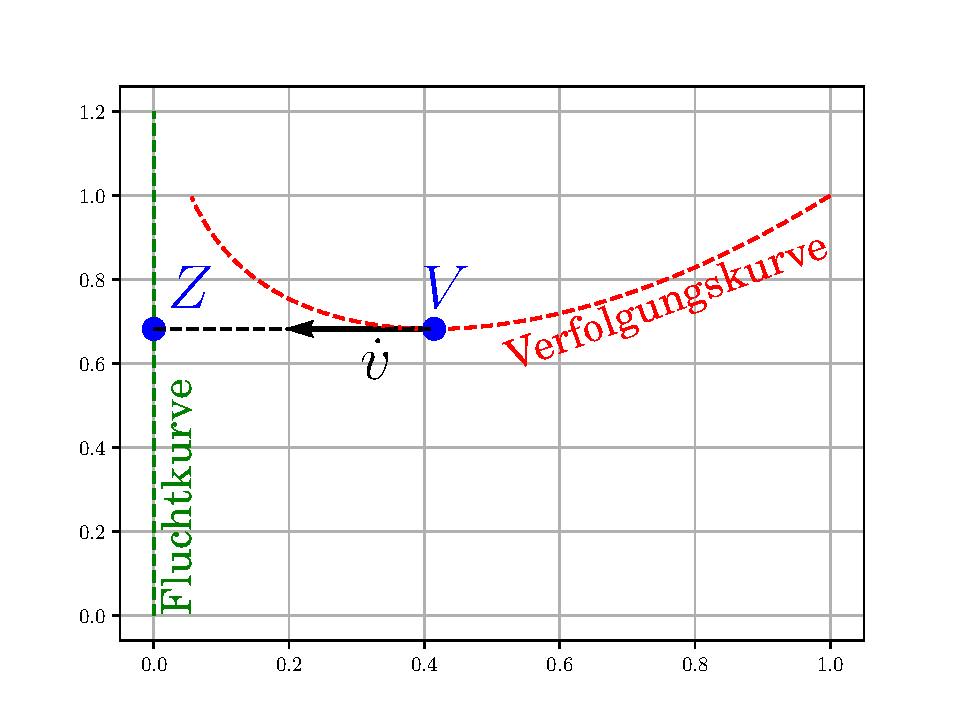
\includegraphics[scale=0.7]{./papers/lambertw/Bilder/Intuition.pdf}
	\caption{Intuition}
	\label{lambertw:grafic:intuition}
\end{figure}
%
Dieses Argument kann leicht überprüft werden, indem lokal alle relevanten benachbarten Punkte betrachtet und das Vorzeichen der Änderung des Abstandes überprüft wird.
Dafür wird ein Ausdruck benötigt, der den Abstand und die benachbarten Punkte beschreibt.

$\dot{v}$ wird allgemein mit dem Winkel $\alpha \in[ 0, 2\pi)$ beschrieben, um alle unmittelbar benachbarten Punkte prüfen zu können.
Die Ortsvektoren der Punkte können wiederum mit
\begin{align}
	v
	&=
	t\cdot\left(\begin{array}{c} \cos (\alpha) \\ \sin (\alpha) \end{array}\right) +\left(\begin{array}{c} x_0 \\ 0 \end{array}\right)
	\\
	z
	&=
	\left(\begin{array}{c} 0 \\ t \end{array}\right)
\end{align}
beschrieben werden.
$x_0$ ist der Abstand bei $t=0$, damit alle möglichen Fälle untersucht werden können.
Da der Abstand allgemein
\begin{equation}
	a
	=
	|v-z|
	\geq
	0
\end{equation}
ist, kann durch Quadrieren ohne Informationsverlust die Rechnung vereinfacht werden zu
\begin{equation}
	a^2
	=
	|v-z|^2
	=
	(t\cdot\cos(\alpha)+x_0)^2+t^2(\sin(\alpha)-1)^2
	\text{.}
\end{equation}
Der Abstand im Quadrat abgeleitet nach der Zeit ist
\begin{equation}
	\frac{d a^2}{d t}
	=
	2(t\cdot\cos (\alpha)+x_0)\cdot\cos(\alpha)+2t(\sin(\alpha)-1)^2
	\text{.}
\end{equation}
Da nur die unmittelbar benachbarten Punkten von Interesse sind, wird die Ableitung für $t=0$ untersucht. Dabei kann die Ableitung in 
\begin{align}
	\frac{d a^2}{d t}
	&=
	2x_0\cos(\alpha)
	\\
	\frac{d a^2}{d t}
	&<
	0\Leftrightarrow\alpha\in\left( \frac{\pi}{2}, \frac{3\pi}{2}\right)
	\\
	\frac{d a^2}{d t}
	&>
	0\Leftrightarrow\alpha\in\left[0, \frac{\pi}{2}\right)\cup\left(\frac{3\pi}{2}, 2\pi\right)
	\\
	\frac{d a^2}{d t}
	&=
	0\Leftrightarrow\alpha\in\left\{ \frac{\pi}{2}, \frac{3\pi}{2}\right\}
\end{align}
unterteilt werden.
Von Interesse ist lediglich das Intervall $\alpha\in\left( \frac{\pi}{2}, \frac{3\pi}{2}\right)$, da der Verfolger sich stets in die negative $y$-Richtung bewegt.
In diesem Intervall ist die Ableitung negativ, woraus folgt, dass jeglicher unmittelbar benachbarte Punkt, den der Verfolger als nächstes begehen könnte, stets näher am Ziel ist als zuvor.
Dies bedeutet, dass der Scheitelpunkt der Verfolgungskurve nie ein lokales Minimum bezüglich des Abstandes sein kann.
%
\subsection{Wo ist der Abstand minimal?}
Damit der Verfolger das Ziel erreicht muss die Bedingung \eqref{lambertw:minimumAbstand} erfüllt sein.
Somit ist es ausreichend zu zeigen, dass
\begin{equation}
    \operatorname{min}(|z-v|)<a_\text{min}
    \label{lambertw:Bedingung:abstandMinimal}
\end{equation}
erfüllt ist.

Für folgende Betrachtung wurde für den Verfolger die Jagdstrategie mit $|\dot{v}|=|\dot{z}|$ gewählt.
Das Minimum des Abstandes kann mit
\begin{equation}
    0=\frac{d|z-v|}{dt}
\end{equation}
gefunden werden.
Mithilfe $(z-v)(z-v)=|z-v|^2$ kann die Gleichung umgeformt werden zu
\begin{equation}
    0=\frac{d(\sqrt{(z-v)(z-v)})}{dt}
    \text{.}
\end{equation}
Jetzt kann die Ableitung leicht ausgeführt werden, womit
\begin{equation}
    0=(\dot{z}-\dot{v})\frac{z-v}{\sqrt{(z-v)(z-v)}}
\end{equation}
entsteht.
In dieser Gleichung kann $(z-v)(z-v)=|z-v|^2$ nochmals angewendet werden, wodurch die Gleichung zu
\begin{equation}
    0=(\dot{z}-\dot{v})\frac{z-v}{|z-v|}
\end{equation}
umgeformt werden kann.
Nun ist die Struktur der Gleichung \eqref{lambertw:richtungsvektor} erkennbar.
Wird dies ausgenutzt folgt
\begin{equation}
    0=(\dot{z}-\dot{v})\frac{\dot{v}}{|\dot{v}|}
    \text{.}
\end{equation}
Durch algebraische Umwandlung kann die Gleichung in die Form
\begin{equation}
    \dot{z}\dot{v}=|\dot{v}|^2
\end{equation}
gebracht werden.
Wenn für den Winkel zwischen den Richtungsvektoren $\alpha$ und die Eigenschaft $|\dot{z}|=|\dot{v}|$ verwendet wird entsteht
\begin{equation}
    \cos(\alpha)=1
    \text{.}
\end{equation}
Jetzt ist klar, dass nur bei $\alpha=0$, wenn $\alpha \in [0,2\pi)$, ein lokales als auch globales Minimum vorhanden sein kann.
$\alpha=0$ bedeutet, dass $\dot{v}=\dot{z}$ sein muss.
Da die Richtungsvektoren bei $t\rightarrow\infty$ immer in die gleiche Richtung zeigen ist dort die Bedingung immer erfüllt.
Dies entspricht gerade dem einen Rand von $t$, der andere Rand bei $t=0$ muss auch auf lokales bzw. globales Minimum untersucht werden.
Daraus folgt, dass die Bedingung \eqref{lambertw:Bedingung:abstandMinimal} lediglich für den Abstand bei $t=\{0, \infty\}$ überprüft werden muss.